\chapter{Die Basics}
\pagestyle{empty}

Im Ersten Kapitel werden wir die Grundlagen der Programmierung lernen.

Wir werden rausfinden, was ein Compiler ist, wie ein Programm abläuft und wie man es startet. Wir werden Benutzereingaben verarbeiten und Ausgaben an den Benutzer geben. Wir lassen den Computer Rechnungen für uns anstellen und lernen, was der Kontrollfluß ist - und wie man ihn beeinflusst. Zuletzt werden wir Arrays kennenlernen und unser erstes nützliches Progamm schreiben.

\lesson{Hello world}

Die erste Lektion beschäftigt sich alleine mit der Frage, was eigentlich eine
Programmiersprache überhaupt ist und wie wir den Computer dazu bringen können,
daraus etwas zu machen, was er ausführen kann.  In guter alter
Programmiertradition tun wir das an dem simpelsten aller Programme: Einem, was
einfach nur ein „Hallo Welt!“ ausgibt.

Wie bringen wir also den Computer dazu, diese Ausgabe zu generieren? Dass er
keine natürliche Sprache versteht, sollte klar sein - intern besteht er aus
lauter Transistoren (wenn ihr nicht wisst, was das ist, denkt an winzige
Schalter), die nur die Zustände „an“ und „aus“ kennen, wir müssen also die
Anweisung „gebe Hallo Welt aus“ in ein Format übersetzen, was nur „an“ und
„aus“ benutzt.

Früher wurde genau dies benutzt - meistens über Lochkarten, die vom Computer
gelesen wurden, „ein Loch“ war dann zum Beispiel ein „an“ und „kein Loch“ war
„aus“, so wurde dann das Programm in Reihen angeordnet und jede Reihe entsprach
einem Befehl oder einem Parameter für diesen Befehl.  Dieses Format nennt sich
„Maschinensprache“ und ist immer noch das, was wir heute dem Computer
übergeben, nur, dass wir keine Lochkarten mehr benutzen, sondern Dateien, in
denen lange Ströme von codierten 0en und 1en stehen.

Nun kann man sich vorstellen, dass es ganz schön anstrengend ist, ein
umfangreiches Programm in 0en und 1en zu beschreiben. Deswegen benutzt man
heutzutage so genannte Hochsprachen, um Programme zu beschreiben. Wir
beschreiben also den Programmablauf in einer von Menschen lesbaren und
verstehbaren Sprache -- wir benutzen hier \Cpp.  Die Programmbeschreibung in
\Cpp legen wir dabei in einer Textdatei ab, meistens hat diese die Endung
\texttt{.cpp}.

Diese Beschreibung des Programms übergeben wir dann an einen \emph{Compiler},
der daraus dann Maschinencode generiert, den wir wiederum dem Computer zur
Ausführung geben können.  Der Compiler für \Cpp, den wir in diesem Kurs
benutzen wollen, heißt \texttt{g++}.

Dem Compiler übergeben wir die zu kompilierende Datei als Parameter, indem wir
sie im Terminal dahinter schreiben:
\begin{center}
\texttt{g++ zuKompilierendeDatei.cpp}
\end{center}
Wir können zusätzlich den Namen der Ausgabedatei festlegen, indem wir vor diese
ein \texttt{-o} (o für output) schreiben:
\begin{center}
\texttt{g++ -o outputDatei zuKompilierendeDatei.cpp}
\end{center}

Nachdem \texttt{g++} uns also ein Maschinencodefile \texttt{outputDatei}
erzeugt hat, können wir es zur Ausführung bringen. Wir tun das, indem wir in
einem Terminal
\begin{center}
	\texttt{./outputDatei}
\end{center}
eingeben, also einen Punkt, ein Slash und dann den Dateinamen.

Zur besseren Übersichtlichkeit hier der ganze Vorgang noch mal in einem
Diagramm:

% TODO: Buttugly, but well...
\begin{center}
    \resizebox{\textwidth}{!}{
        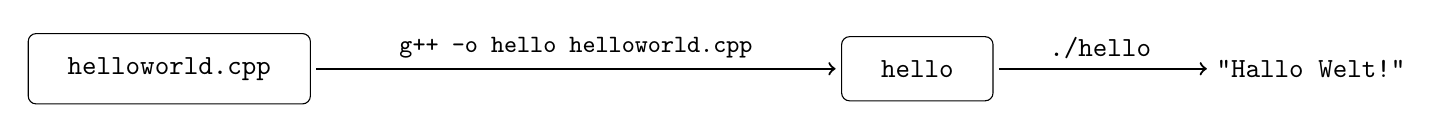
\begin{tikzpicture}
            \node (nHelloWorldCpp) [ shape=rectangle, rounded corners = 0.1cm, draw=black, inner xsep=0.5cm, inner ysep = 0.3cm ] {\texttt{helloworld.cpp}};
            \node (nHello) [ right of = nHelloWorldCpp, node distance = 9.5cm, shape=rectangle, rounded corners = 0.1cm, draw = black, inner xsep = 0.5cm, inner ysep = 0.3cm ] {\texttt{hello}};
            \draw [->, thick, shorten >= 2pt, shorten <= 2pt ] (nHelloWorldCpp) -- (nHello) node [ midway, above, font = \small ] { \texttt{g++ -o hello helloworld.cpp}} ;
            \node (nOutput) [ right of = nHello, node distance = 5cm, shape=rectangle ] {\texttt{"Hallo Welt!"}};
            \draw [->, thick, shorten <= 2pt] (nHello) -- (nOutput) node [ midway, above ] {\texttt{./hello}};
        \end{tikzpicture}
    }
\end{center}

\textbf{Praxis:}
\begin{enumerate}
	\item Öffnet ein Terminal, ihr findet dies in den Anwendungen (oben rechts)
		unter „Systemwerkzeuge“
    \item Wechselt in das Verzeichnis \texttt{vorkurs/lektion01}, indem ihr
		\texttt{cd vorkurs/lektion01}\footnote{was dieser Befehl genau tut und wie er funktioniert, erfahrt ihr in Lektion 2} eingebt und enter drückt.
    \item In diesem Verzeichnis liegt eine Datei \texttt{helloworld.cpp}.
        Benutzt \texttt{g++}, um diese zu einer Datei \texttt{hello} zu
        kompilieren. Orientiert euch dazu an den Befehlen von oben.
    \item Führt die Datei \texttt{hello} aus.
\end{enumerate}

\inputcpp{helloworld.cpp}

\textbf{Spiel:}

Ihr könnt nun versuchen, den Quellcode selbst zu verändern und damit ein wenig
herumzuspielen. Öffnet dazu einen Editor (in den Anwendungen findet ihr z.B.
unter „Zubehör“ den Editor gedit) und öffnet die Datei
\texttt{vorkurs/lektion01/helloworld.cpp}\footnote{entweder mittels
"Datei/Öffnen" in gedit oder über das Terminal mittels \texttt{gedit
helloworld.cpp}}. Denkt daran, nach jeder Änderung die Datei zu speichern und
im Terminal neu zu kompilieren und auszuführen.

Dinge, die ihr ausprobieren könntet sind zum Beispiel:
\begin{enumerate}
    \item Was passiert, wenn ihr „Hello world!“ in etwas anderes ändert?
    \item Was passiert, wenn ihr die erste Zeile löscht (der Originalquellcode
        ist in diesem pdf enthalten, ihr könnt sie also später wieder
        herstellen)?
    \item Was passiert, wenn ihr das „\verb|<< std::endl|“ löscht?
    \item Wie könnte man mehrere Sätze ausgeben? Wie könnte man mehrere Zeilen
        ausgeben?
\end{enumerate}

\lesson{Die Shell}

Wenn ihr bisher nur mit Windows oder Mac gearbeitet habt, habt ihr
wahrscheinlich in der letzten Lektion nebenbei etwas neues Kennen gelernt: Die
Shell.

Auch wenn sich unter Linux zunehmend Desktopumgebungen, wie man sie von
kommerziellen Betriebssystemen kennt verbreiten, bleibt die Shell immer noch das
Mittel der Wahl, wenn man sich mit dem System auseinander setzen, oder auch
allgemein arbeiten will. Wir erachten zumindest die Shell als wichtig genug, um
euch direkt zu beginn damit zu konfrontieren.

Wann immer ihr über das Anwendungsmenü ein Terminal startet, wird dort drin
automatisch auch eine shell gestartet. Die beiden Konzepte sind tatsächlich so
eng miteinander verknüpft, dass ihr euch um die Unterschiede erst einmal keine
Gedanken machen müsst - wann immer ihr Shell oder Terminal hört, denkt einfach
an das schwarze Fenster mit dem Text. Das ist auch das wesentliche Merkmal der
Shell, sie ist ein Textbasiertes interface zu eurem Computer. Ihr gebt Befehle
ein, sie gibt euch Text zurück und auf diese Weise könnt ihr eigentlich alles
machen, was ihr sonst gewohnterweise mit der Maus und grafischen Oberflächen
tun würdet.

Wenn die Shell auf eure Befehle wartet, zeigt sie euch den so genannten
\emph{Prompt} an. Er enthält unter anderem euren Nutzernamen und das aktuelle
Verzeichnis (\verb|~| steht dabei für euer Nutzerverzeichnis, ein spezieller
Ordner, der eurem Account zugeordnet ist und in dem ihr alle Rechte besitzt).

Wenn ihr in ein anderes Verzeichnis wechseln wollt, könnt ihr das (wie ihr
bereits in der ersten Lektion gelernt habt) mit dem Befehl \texttt{cd} tun,
gefolgt von dem Namen des Verzeichnis. Um zurück zu gehen, könnt ihr das
spezielle Verzeichnis \texttt{..} (also zwei Punkte) angeben, welches für das
nächst höher liegende Verzeichnis steht. Wenn ihr euch den Inhalt des
Verzeichnisses anschauen wollt, könnt ihr dafür den Befehl \texttt{ls}
benutzen. Um herauszufinden, in welchem Verzeichnis ihr euch befindet, könnt
ihr \texttt{pwd} nutzen, zum Kompilieren von C++-Programmen habt ihr den Befehl
\texttt{g++} kennengelernt. Solltet ihr Hilfe zu irgendeinem Befehl benötigen,
könnt ihr den Befehl \texttt{man} (für „Manual“) geben, gefolgt von dem Befehl,
zu dem ihr Hilfe braucht (über \texttt{man} werden wir später noch
ausführlicher reden).

\textbf{Praxis:}
\begin{enumerate}
    \item Öffnet ein Terminal und gebt die folgenden Befehle ein:
    \inputshell{basics.sh}
\end{enumerate}

\textbf{Spiel:}
\begin{enumerate}
    \item Versucht selbst, euer Nutzerverzeichnis (\emph{home}) zu navigieren.
        Wie viele Lektionen hat der Vorkurs?
    \item Was passiert, wenn ihr euer Homeverzeichnis verlasst (\texttt{cd ..}
        während ihr darin seid)?
    \item Versucht in der manpage von ls (\texttt{man ls}) zu stöbern und die
        verschiedenen Parameter, mit denen ihr das Verhalten steuern könnt zu
        erforschen. Findet ihr heraus, wie ihr ein longlisting anzeigen lässt,
        in dem unter anderem auch die Dateigröße zu jeder Datei steht?
\end{enumerate}

\lesson{Input und Output}

Nachdem wir ein bisschen Vertrauen in die shell entwickelt haben und zumindest
bereits unser erstes Programm kompiliert, wollen wir nun etwas spannendere
Dinge tun. Nach wie vor müsst ihr nicht jede Zeile eures Programmes verstehen.
Sollte euch bei einer bestimmten Zeile trotzdem interessieren, was genau sie
tut, versucht doch eventuell sie zu entfernen, das Programm zu kompilieren und
schaut, was sich ändert.

Wir wollen uns nun mit grundlegendem input und output vertraut machen, denn
erst wenn euer Programm mit einer Benutzerin interagiert, wird es wirklich
nützlich. Wir haben in der ersten Lektion bereits \texttt{cout} (für
\emph{console out}) kennengelernt, um Dinge auszugeben. Nun nutzen wir
\texttt{cin}, um Eingaben des Benutzers entgegen zu nehmen. Jedes Programm
unter Linux (und übrigens auch Mac OS oder Windows) kann auf diese Weise
Eingaben von der Nutzerin entgegen nehmen und Ausgaben liefern. Das ist auch
der Grund, warum die Konsole so wichtig ist und es viele Dinge gibt, die nur
mittels einer Konsole gelöst werden können: Während es viele Stunden dauert,
ein grafisches Interface zu programmieren, über die man mit dem Programm mit
der Maus kommunizieren kann, kann praktisch jeder ein textbasiertes
Konsoleninterface schreiben. Linux ist ein Ökosystem mit einer gewaltigen
Anzahl tools für jeden denkbaren Zweck und bei den meisten haben die Autorinnen
sich nicht die Mühe gemacht, extra eine grafische Oberfläche zu entwickeln.

Nun aber direkt zur Praxis:

\textbf{Praxis:}
\begin{enumerate}
    \item Öffnet die Datei \texttt{vorkurs/lektion03/helloyou.cpp} in eurem Texteditor
    \item Öffnet ein Terminal und wechselt in das Verzeichnis \texttt{vorkurs/lektion3}
    \item Kompiliert im Terminal die Datei (\texttt{g++ -o helloyou
        helloyou.cpp}) und führt sie aus (\texttt{./helloyou})
    \item Versucht verschiedene Eingaben an das Programm und beobachtet, was passiert
\end{enumerate}

\inputcpp{helloyou.cpp}

\textbf{Spiel:}

\begin{enumerate}
    \item Versucht, zu verstehen, was die einzelnen Teile des Programms tun. An
        welcher Stelle erfolgt die Eingabe? Was passiert dann damit?
    \item Erweitert das Programm um eigene Fragen und Ausgaben. Vergesst nicht,
        dass ihr das Programm nach jeder Änderung neu kompilieren und testen
        müsst.
\end{enumerate}

\lesson{Fehlermeldungen und häufige Fehler}

Wenn ihr in den vergangen Lektionen ein bisschen herumprobiert habt, wird es
euch sicher das ein oder andere mal passiert sein, dass euch der Compiler statt
eines funktionierenden Programms eine Riesenmenge Fehlermeldungen ausgespuckt
hat und ihr einen Schreck bekamt und schon dachtet, ihr hättet alles kaputt
gemacht.

\texttt{g++} ist leider bei Fehlermeldungen immer sehr ausführlich und gibt
euch lieber viel zu viel, als viel zu wenig aus. Das kann im ersten Blick ein
bisschen überwältigend wirken, aber wenn man einmal gelernt hat, wie die
Fehlermeldungen am Besten zu lesen sind, ist das alles gar nicht mehr so
schlimm.

Wir schieben deswegen eine Lektion über häufige Fehlerquellen ein und wie man
Fehlermeldungen von \texttt{g++} liest, um möglichst schnell die Ursache des
Fehlers zu finden.

Nehmen wir z.B. mal folgendes Programm:

\inputcpp{fehler1.cpp}

Wenn wir versuchen, dieses zu kompilieren, gibt uns \texttt{g++} folgendes aus:

\begin{textcode*}{label=g++ -o fehler1 fehler1.cpp}
fehler1.cpp: In function 'int main()':
fehler1.cpp:2:5: error: 'cout' is not a member of 'std'
fehler1.cpp:2:35: error: 'endl' is not a member of 'std'
\end{textcode*}

Wenn wir diese Fehlermeldung verstehen wollen, fangen wir immer ganz oben an,
egal wie viel Text uns der Compiler ausspucken mag. In diesem Fall sagt uns die
erste Zeile, in welcher Datei (\texttt{fehler1.cpp}) der Fehler aufgetreten ist
und in welcher Funktion (\texttt{int main()}). Die beiden Zeilen
danach sind sogar noch spezifischer: Sie enthalten zu Beginn den Dateinamen,
dann einen Doppelpunkt, gefolgt von einer Zeilennummer, gefolgt von einer
Spaltennummer. Das gibt euch ganz genau die Stelle an, an der der Compiler
etwas an eurem Code zu bemängeln hat. In diesen Fall ist, was der Compiler
bemängelt, dass \texttt{cout} bzw. \texttt{endl} nicht in \texttt{std} sind.
Was genau \texttt{std} bedeutet muss uns nicht interessieren, aber der Rest
sagt uns (mit ein bisschen Erfahrung) dass wir die Definition von \texttt{cout}
und \texttt{endl} nicht haben - was nicht weiter verwunderlich ist, denn diese
beiden Dinge werden in der Datei \texttt{iostream} definiert, die wir früher
immer includiert haben.

Damit wissen wir jetzt auch (endlich) was das \mint{c++}|#include <iostream>|
zu bedeuten hatte. Offenbar brauchen wir das, wenn wir Konsolen input und
output machen wollen, da es die Definitionen von \texttt{cout}, \texttt{cin},
\texttt{endl} und ähnlichem enthält.

Der nächste sehr häufig vorkommende Fehler ist subtiler:

\inputcpp{fehler2.cpp}

Wenn wir versuchen, dies zu kompilieren, bekommen wir vom Compiler
entgegengespuckt:

\begin{textcode*}{label=g++ -o fehler2 fehler2.cpp}
fehler2.cpp: In function 'int main()':
fehler2.cpp:5:1: error: expected ';' before '}' token
\end{textcode*}

Wiederum sagt uns die erste Zeile, in welcher Datei und Funktion der Fehler
aufgetreten ist. Die zweite Zeile sagt uns wo, nämlich in Zeile 5, direkt am
Anfang. Die Beschwerde des Compilers ist, dass er ein Semikolon erwartet hat,
aber eine geschlossene geschweifte Klammer gefunden hat. Der Grund dafür ist,
dass in \Cpp erwartet wird, dass jede Anweisung mit einem Semikolon abgeslossen
wird.  Wenn ihr euch die bisherigen Quellcodedateien anschaut, werdet ihr
feststellen, dass hinter den allermeisten Zeilen ein solches Semikolon steht.
Hier fehlt es allerdings nach der Ausgabe in Zeile 4. Sobald wir es hinzufügen,
beschwert sich der Compiler nicht mehr.

Hier zeigt sich eine ein bisschen verwirrende Angewohnheit von Fehlermeldungen
von \Cpp: Obwohl der Compiler behauptete, der Fehler läge in Zeile 5, lag er in
Wahrheit bereits in Zeile 4. Hier müsst ihr dem dummen Compiler ein wenig
nachsichtig sein - er kann es einfach nicht besser wissen. Wenn ihr also mal in
der richtigen Zeilennummer nachschlagt, aber nicht wisst, wo dort der Fehler
sein sollte, schaut vielleicht mal ein oder zwei Zeilen darüber, vielleicht
wusste der Compiler es einfach nicht besser.

\textbf{Praxis:}
\begin{enumerate}
    \item Versucht, folgende Dateien zu kompilieren und schaut euch die
        Fehlermeldung an. In welcher Zeile, in welcher Spalte liegt der Fehler?
        Was gibt euch der Compiler als Fehlermeldung aus?
    \item Versucht, die aufgetretenen Fehler zu korrigieren. Bekommt ihr es
        hin, dass der Compiler sich nicht mehr beschwert und das Programm
        korrekt arbeitet (schaut euch ggf. die bisher gezeigten Quellcodes an)?
\end{enumerate}

\inputcpp{fehler3.cpp}
\inputcpp{fehler4.cpp}

\textbf{Spiel:}
\begin{enumerate}
    \item Das folgende Programm enthält mehrere Fehler. Bekommt ihr trotzdem
        raus, welche das sind und könnt ihr sie beheben (Tipp: „c++ math“ zu
        \href{http://lmgtfy.com/?q=c\%2B\%2B+math}{googlen} kann euch hier vielleicht weiter bringen)?
    \item Wenn ihr in den Vergangen Lektionen ein bisschen gespielt habt und
        vereinzelnd versucht habt, Dinge zu löschen, Werden euch viele
        Fehlermeldungen begegnet sein, versucht, diese zu lesen und
        interpretieren, was euch der compiler hier sagen will.
\end{enumerate}

\inputcpp{fehler5.cpp}

\lesson{Variablen}

Das Programm \texttt{variablen.cpp} erzählt von ihrem Tag.
Compilier es und guck dir die Ausgabe an.

\inputcpp{variablen.cpp}

Da immer wieder das gleiche Wort \glqq{}wundervoll\grqq{} benutzt wird, wurde es in eine sogenannte \emph{Variable} ausgelagert.
Eine Variable ist ein Wert der mit einem Namen benannt wird.
Dabei findet die Zuweisung durch ein \cppinline{=} statt, dem Namen auf der linken Seite des Gleichheitszeichen wird der Wert auf der rechten Seite zugewiesen.
Im Programm selbst ist es dann so, als würde der Wert an der Stelle des Namens stehen.

Der Wert einer Variable kann sich im Laufe des Programmes verändern.
Durch Hinzufügen der Zeile \cppinline{beschreibung = "langweilig";} wird hinter dieser Zeile anstelle von \glqq{}wundervoll\grqq{} nun \glqq{}langweilig\grqq{} ausgegeben.
Ähnlich kann wie in \texttt{helloyou.cpp} der Wert von Variablen durch \cppinline{std::cin >> beschreibung} die Benutzerin eingeben werden.

Variablen haben immer einen bestimmten \emph{Datentypen}.
In unserem Beispiel handelt es sich um \cppinline{std::string}.
Der Datentyp wird bei dem Erstellen -- also der ersten Zuweisung -- vor dem Namen angeben.
Dieser wird benötigt, damit der Computer weiß, um was für eine Art Wert es sich handelt -- ein Text sollte anders behandelt werden als eine Zahl.
Beispielsweise kann man zwei Zahlen miteinander multiplizieren, für Texte ergibt das allerdings keinen Sinn.
In der Lektion Arithmetik lernen wir mehr über Zahlen und deren Eigenheiten.

\textbf{Praxis:}
\begin{enumerate}
    \item Was passiert, wenn ihr \cppinline{beschreibung} in Zeile 5 ein anderes Wort zuweist?
    \item Definiert eine weitere Variable und schreibt einen weiteren Satz.
\end{enumerate}

\textbf{Spiel:}
\begin{enumerate}
    \item Was passiert, wenn ihr euch im Namen einer Variable „vertippt“?
    \item Definiert euch zwei \cppinline{std::string} Variablen, weist ihnen
        irgendwelchen Text zu, versucht, sie zu addieren und das Ergebnis auszugeben.
    \item Was passiert, wenn ihr eine \cppinline{std::string} Variable definiert,
        ihr aber nichts zuweist und dann versucht, sie auszugeben?
\end{enumerate}

\lesson{Manpages}

Wir machen eine kurze Pause vom \Cpp und schauen uns in der Zwischenzeit
\emph{man pages} an. Wie wir bereits fest gestellt haben, kann man diese
benutzen, um sich mehr Informationen über Befehle anzeigen zu lassen. Wir
wollen uns jetzt genauer anschauen, wie man all die Informationen in einer man
page am Besten konsumiert.

Wir schauen uns das am Beispiel der Manpage \texttt{man cp} an (\texttt{cp} ist
der Befehl zum Kopieren von Dateien).

\textbf{Praxis:}
\begin{enumerate}
    \item Öffnet eine Konsole und gebt \texttt{man cp} ein.
\end{enumerate}

Die man page besteht aus mehreren \emph{Sections}. Welche sections genau es
gibt, hängt von der man page ab, aber meistens gibt es mindestens die folgenden
sections:
\begin{description}
    \item[\texttt{NAME}]
        Gibt euch den Namen des Befehls und eine Einzeilige Beschreibung an
    \item[\texttt{SYNOPSIS}]
        Gibt euch die generelle Benutzung des Befehls an. In diesem Fall gibt
        es drei mögliche Formen. Allen gemein ist, dass man zunächst
        \texttt{cp} eingibt, darauf folgen Optionen. Wie der Rest interpretiert
        wird, hängt dann vom Rest ab. Werden zwei weitere Parameter angegeben,
        wird der erste als Quelle, der zweite als Ziel interpretiert (erste
        Form). Werden mehr Parameter angegeben, wird das letzte als
        Verzeichnis, in das man alle anderen kopieren will interpretiert
        (zweite Form). In der dritten Form (wenn \texttt{-t} angegeben wird)
        wird hingegen der \emph{erste} Parameter als das Zielverzeichnis
        interpretiert, in das alle anderen Dateien kopiert wird.

        Es gibt eine Vielzahl von Konventionen für diesen Bereich, eckige
        Klammern bedeuten z.B. dass dieser Teil auch weggelassen werden darf,
        drei Punkte bedeuten, dass hier mehrere solche Dinge stehen können.

        Dieser Bereich ist der, der am Interessantesten für euch ist, wenn ihr
        „einfach schnell wissen wollt, wie es funktioniert“.
    \item[\texttt{DESCRIPTION}]
        Hier wird ausführlicher beschrieben, was der Befehl tut. Hier werden
        auch alle möglichen Optionen beschrieben, die wir dem Befehl bei
        \texttt{[OPTION]...} mitgeben können. Die wichtigen Informationen
        stehen meistens irgendwo in diesem Bereich.
    \item[\texttt{AUTHOR}, \texttt{REPORTING BUGS}, \dots]
        Hier stehen weitere Hintergrundinformationen, die meistens eher für
        Entwicklerinnen interessant sind.
    \item[\texttt{SEE ALSO}]
        Auch eine wichtige section für euch: Wenn ihr die gewünschte
        Information nicht gefunden habt, oder ihr nicht den richtigen Befehl
        gefunden habt, stehen hier manchmal verwandte Befehle oder Quellen
        weiterer Informationen.
\end{description}

Man pages sind häufig sehr umfangreich und enthalten viel mehr Informationen,
als ihr euch gerade wünscht. Es ist nicht immer einfach, die gerade relevanten
Informationen heraus zu filtern und es gibt nichts frustrierenderes, als einen
Befehl gerade dringend zu brauchen, aber nicht zu kennen und sich erst durch
eine lange man page lesen zu müssen.

Dennoch ist es eine sehr hilfreiche Fähigkeit, zu wissen, wie man man pages
liest und sich einfach in einem ruhigen Moment mal durch die ein oder andere
man page durch zu lesen. Häufig lernt man dabei neue Dinge, manchmal macht es
einem das Leben irgendwann sehr viel leichter, sie zu wissen.

Habt von daher Geduld, wenn euch eine wirsche Linux-Expertin auf die Frage, wie
ihr unter Linux euren Laptop in den Ruhemodus versetzt ein schnelles „man
pm-suspend“ antwortet. Mit ein bisschen Übung wird euch das tatsächlich
hinreichend schnell zur richtigen Lösung verhelfen.

\textbf{Praxis:}
\begin{enumerate}[resume]
    \item Öffnet die man page von \texttt{ls}. Findet die Optionen zur langen
        Listung, zum Sortieren nach Dateigröße und um auch versteckte Dateien
        (unter Linux sind das alle, die mit \texttt{.} anfangen) anzuzeigen und
        probiert sie aus.
    \item Was ist der Unterschied zwischen \texttt{ls -a} und \texttt{ls -A}?
        Probiert beides aus.
    \item Nutzt \texttt{cp} um eine Datei zu kopieren. Sucht euch dafür
        irgendeine \texttt{.cpp}-Datei aus dem Vorkurs-Programm und kopiert sie
        in euer Homeverzeichnis (ihr könnt dafür eine Tilde (\texttt{\~})
        benutzen).
\end{enumerate}

\textbf{Spiel:}
\begin{enumerate}
    \item Wie über so gut wie jeden Befehl gibt es auch über \texttt{man} eine
        manpage. Schaut euch mal \texttt{man man} an.
    \item Befehle, die für euch im späteren Leben interessant sein könnten sind
        z.B. \texttt{tar}, \texttt{mkdir}, \texttt{grep}, \texttt{cat},
        \texttt{echo}, \texttt{mv}, \dots. Ihr könnt ja schon einmal in ein
        oder zwei dieser manpages hinein schauen, und ein oder zwei Befehle
        ausprobieren.
\end{enumerate}

\lesson{Arithmetik}

Wir haben in der vergangenen Lektion Variablen vom Typ \texttt{std::string}
kennengelernt. Zeichenketten zu speichern ist schon einmal ein guter Anfang,
aber wir wollen auch rechnen können, wir brauchen also mehr Typen für
Variablen.

\Cpp unterstützt eine Unmenge an Datentypen und hat auch die Möglichkeit,
eigene zu definieren. Wir wollen uns hier nur mit den Wichtigsten beschäftigen.

Fangen wir mit dem wohl meist genutzten Datentyp an: Einem \texttt{int}, oder
\texttt{integer}. Dieser speichert eine ganze Zahl (mit bestimmten Grenzen, an
die wir aber erst einmal nicht stossen werden, von daher ignorieren wir sie
erst einmal frech). Mit \texttt{int}s können wir rechnen, das funktioniert in
\Cpp mit ganz normalen Rechenausdrücken, wie wir sie aus der Schule kennen,
plus den bereits angetroffenen Zuweisungen:

\inputcpp{arith1.cpp}

Wichtig ist hier, zu beachten, dass wir dem Computer ein in Reihenfolge
abgearbeitetes Programm geben, keine Reihe von Aussagen. Das bedeutet in diesem
konkreten Fall, dass wir z.B. nicht die Aussage treffen „\texttt{a} ist gleich
5“, sondern dass wir sagen „lasse zuerst \texttt{a} den Wert 5 haben. Lasse
dann \texttt{b} den Wert 18 haben. Lasse dann \texttt{c} den Wert haben, der
heraus kommt, wenn man den Wert von \texttt{b} vom Wert von \texttt{a}
abzieht“. Besonders deutlich wird dieser Unterschied bei einem Beispiel wie
diesem:

\inputcpp{arith2.cpp}

\textbf{Praxis:}
\begin{enumerate}
    \item Was gibt dieses Programm aus? Überlegt es euch zuerst und kompiliert
        es dann, um es auszuprobieren.
\end{enumerate}

Obwohl \texttt{a = a + 19} mathematisch überhaupt keinen Sinn ergibt, ist doch
klar, was passiert, wenn man sich den Quellcode eben nicht als Reihe von
Aussagen, sondern als Folge von \emph{Anweisungen} vorstellt. Das
Gleichheitszeichen bedeutet dann nicht, dass beide Seiten gleich sein sollen,
sondern dass der Wert auf der linken Seite den Wert auf der rechten Seite
annehmen soll.

Wie wir in diesem Beispiel ausserdem sehen, können wir nicht nur Strings
ausgeben, sondern auch Zahlen. \texttt{std::cout} gibt sie in einer Form aus,
in der wir etwas damit anfangen können. Genauso können wir auch über
\texttt{std::cin} Zahlen vom Benutzer entgegen nehmen:

\inputcpp{arith3.cpp}

Langsam aber sicher tasten wir uns an nützliche Programme heran!

\textbf{Praxis:}
\begin{enumerate}[resume]
    \item Schreibt ein Programm, welches von der Nutzerin zwei ganze Zahlen
        entgegen nimmt und anschließend Summe, Differenz, Produkt und Quotient
        ausspuckt.
    \item Was fällt auf, wenn ihr z.B. 18 und 5 eingebt?
	\item Findet heraus (Google ist euer Freund), wie man in \Cpp Division mit
		Rest durchführt und gebt diese zusätzlich zu den bisherigen Operationen
		mit aus\footnote{Falls ihr nicht weiterkommt, hilft euch vielleicht das
		Stichwort „modulo“ oder „modulo-operator“ weiter.}.
    \item Was passiert, wenn ihr als zweite Zahl eine 0 eingebt?
\end{enumerate}

\textbf{Spiel:}
\begin{enumerate}
    \item Findet heraus, was die größte positive (und was die kleinste
        negative) Zahl ist, die ihr in einem \texttt{int} speichern könnt.
        Faulpelze nutzen Google, Lernbegierige versuchen sie experimentell zu
        ermitteln. Was passiert, wenn ihr eine größere Zahl eingebt?
    \item Wir arbeiten bisher nur mit \texttt{int}s für ganze Zahlen. Wenn wir
        mit gebrochenen Zahlen rechnen wollen brauchen wir den Datentyp
        \texttt{double}. Schreibt euer Mini Rechenprogramm so um, dass es statt
        \texttt{int}s nur noch \texttt{double} benutzt und probiert es aus.
        Achtet darauf, dass es Dezimalpunkte und Dezimalkommata gibt, wenn ihr
        überraschende Ergebnisse erhaltet.
\end{enumerate}

\lesson{Der Debugger}

\textbf{Fehlerklassen}

Es ist wichtig, früh zu verstehen, dass es verschiedene Klassen von Fehlern in
einem \Cpp Programm gibt, die sich alle zu unterschiedlichen Zeitpunkten
auswirken. Die Hauptsächliche Klasse von Fehlern, die wir bisher betrachtet
haben, sind \emph{Compilerfehler}. Sie treten - wie der Name nahe legt - zur
Compilezeit auf, also wenn ihr euer Programm kompilieren wollt. Meistens
handelt es sich hier um relativ einfach erkennbare Fehler in der Syntax (wie
zum Beispiel ein vergessenes Semikolon, oder eine vergessene geschweifte
Klammer), um fehlende header (wie die \verb|\#include <...>| heißen) oder um
undefinierte Variablen.

Eine andere, besonders fiese Klasse von Fehlern haben wir in der letzten
Lektion kennengelernt. Wenn wir nämlich durch eine Variable teilen, und in
dieser Variable erst beim Programmlauf (zur \emph{Laufzeit}) eine 0 steht, so
tritt eine so genannte \emph{floating point exception} auf. Der Compiler hat
hier keine Chance, diesen Fehler zu erkennen - er weiß ja nicht, was der
Benutzer später hier eingibt! Da diese Klasse von Fehlern zur Laufzeit auftritt
heißen sie Laufzeitfehler. Und sie sind immer ein Zeichen von fundamentalen
Fehlern im Programm. Sie sind also die am schwersten aufzutreibenden Fehler, da
es keine automatischen Tools gibt, die uns bei ihrer Suche helfen.

\textbf{gdb}

Wir werden (noch) nicht lernen, wie wir den Fehler aus der letzten Lektion
beheben können, aber wir werden ein wichtiges Tool kennen lernen, um
Laufzeitfehler aufzuspüren, damit wir wenigstens wissen, wo wir mit der Lösung
anfangen können: Den \emph{GNU debugger}, oder kurz gdb.

Der Debugger ist eine Möglichkeit, unser Programm in einer besonderen Umgebung
laufen zu lassen, die es uns erlaubt es jederzeit anzuhalten, den Inhalt von
Variablen zu untersuchen oder auch Anweisung für Anweisung unser Programm vom
Computer durchgehen zu lassen.

Damit er das tun kann, braucht er vom Compiler ein paar zusätzliche
Informationen, über den Quellcode, die normalerweise verloren gehen. Wir müssen
dem Compiler dafür ein paar zusätzliche Optionen mitgeben:
\begin{minted}{bash}
g++ -O0 -g3 -o debugger debugger.cpp
\end{minted}
(Beachtet, dass im ersten Parameter erst ein großer Buchstabe o, dann eine 0 stehen)
\inputcpp{debugger.cpp}
\textbf{Praxis:}
\begin{enumerate}
    \item Kompiliert das Programm mit den neuen Optionen für den debugger. Ihr
        könnt es dann mittels \verb|gdb ./debugger| im gdb starten. Ihr solltet
        nun ein wenig Text ausgegeben bekommen und einen anderen prompt. Ihr
        könnt den debugger jederzeit wieder verlassen, indem ihr \texttt{quit}
        eingebt (falls ihr gefragt werdet, ob ihr euch sicher seid, gebt
        \texttt{y} ein und drückt enter)
    \item Zu allererst müssen wir einen so genannten \emph{breakpoint} setzen,
        das ist ein Punkt im Programmablauf, an dem es stoppen soll, damit wir
        entscheiden können, was wir tun wollen. \texttt{main} ist für die
        meisten unserer Programme eine sichere Wahl:
        \mint{text}|break main|
        Dann können wir das Programm mit \texttt{run} starten. Wir sollten die
        erste Anweisung unseres Programmes angezeigt bekommen.
    \item Der Debugger wird euch jetzt immer sagen, welches die nächste
        Anweisung ist, die er ausführen möchte. Mit \texttt{next} könnt ihr sie
        ausführen lassen, mit \texttt{print a} könnt ihr euch den Inhalt von
        \texttt{a} zu diesem Zeitpunkt anschauen, mit \texttt{print b} den von
        \texttt{b} und so weiter. Geht das Programm Schritt für Schritt durch
        und lasst euch die Werte von \texttt{a}, \texttt{b} und \texttt{c} in
        jedem Schritt ausgeben. Wenn der debugger euch sagt, dass euer Programm
        beeendet wurde, gebt \texttt{quit} ein und beendet ihn.
\end{enumerate}

\textbf{Spiel:}
\begin{enumerate}
    \item Ihr habt nun schon einige Programme kennen gelernt. Kompiliert sie
        für den Debugger neu und untersucht sie genauso wie obiges Programm,
        solange ihr Lust habt.
\end{enumerate}

\lesson{Der Kontrollfluss}

Nachdem wir ein bisschen etwas über den Debugger verstanden haben (wir werden
ihn noch häufiger benutzen), können wir uns nun wieder unserem Problem mit der
Division durch 0 zuwenden.

\inputcpp{arith4.cpp}

Wenn wir dieses Programm kompilieren und als zweite Zahl eine 0 eingeben,
werden wir auf der Konsole ausgegeben bekommen:
\begin{minted}{text}
Gebe eine Zahl ein: 5
Gebe noch eine Zahl ein: 0
Floating point exception
\end{minted}
(Gegebenenfalls ist die letzte Zeile bei euch auch in einer anderen Sprache)

Wir können das Programm auch einmal im debugger ausführen und werden wenig
überraschend feststellen, dass die Anweisung, an der diese floating point
exception auftritt die ist, in der die Division steht.

Wenn wir diesen Fehler beheben wollen, haben wir eigentlich nur zwei
Möglichkeiten: Die erste ist, die Schuld auf den Benutzer zu schieben, warum
versucht er auch, eine 0 einzugeben? Ich hoffe, ihr stimmt zu, dass das nicht
seht Benutzerfreundlich wäre. Stellt euch vor, jedes mal, wenn ihr in einem
Programm einen Wert eingibt, auf den das Programm nicht vorbereitet ist, würde
es direkt abstürzen. Das fändet ihr vermutlich nicht so gut, es sollte doch
zumindest mal eine Fehlermeldung ausgeben und den Benutzen informieren, dass er
was falsch gemacht hat.

Und das ist der zweite Weg, den wir jetzt einschlagen wollen. Unser Programm
sollte am Besten, nachdem es die Eingabe vom Benutzer entgegen genommen hat,
einfach überprüfen, ob die Division erlaubt ist oder nicht. Sollte der Benutzer
eine 0 eingegeben haben, sollte es den Benutzer auf seinen Fehler hinweisen und
sich beenden, sonst sollte es den Quotienten ausgeben. Diese Abhängigkeit des
Verhaltens eines Programms von den Eingaben, bezeichnen wir als
\emph{Kontrollfluss}, man kann das mit einem Diagramm verdeutlichen:

\begin{center}
    \begin{tikzpicture}[auto, node distance=3cm,>=latex']
        \tikzstyle{block} = [draw, fill=blue!20, rectangle, minimum height=3em, minimum width=6em]

        \node [block] (start) {Input};
        \node [block, right of=start] (if) { $a=0$? };
        \node [block, right of=if, node distance=4cm] (fehler) { Gib Fehler aus };
        \node [block, below of=fehler,node distance =  2cm] (quotient) { Gib Quotient aus };
        \node [block, right of=fehler, node distance = 3.5cm] (ende) { Ende };

        \draw [->] (start) -- node {} (if);
        \draw [->] (if) -- node {\texttt{ja}} (fehler);
        \draw [->] (if.south) |- node [above, near end] {\texttt{nein}} (quotient);
        \draw [->] (quotient) -| node {} (ende);
        \draw [->] (fehler) -- node {} (ende);
    \end{tikzpicture}
\end{center}

Die einfachste Möglichkeit, den Kontrollfluss zu ändern, besteht in so
genannten „bedingten Anweisungen“:
\inputcpp{if.cpp}

In den Zeilen 12 bis 20 sehen wir, wie eine solche Bedingte Anweisung in \Cpp
aussieht. Wir erkennen relativ direkt unser Diagramm hier wieder: In Zeile 12
steht der „$a=0$?“ Block, in den Zeilen 13 bis 17 steht der „Gib Fehler aus“
Block und in Zeile 19 der „Gib den Quotienten aus“ Block.

Beachtet allerding die doppelten Gleichheitszeichen in Zeile 12. \Cpp hat
getrennte Operatoren für Vergleiche und Zuweisungen - Doppelte
Gleichheitszeichen bedeuten Vergleich („sind diese beiden gleich?“), ein
einfaches Gleichheitszeichen bedeutet Zuweisung („mache diese beiden gleich!“).

\textbf{Praxis:}
\begin{enumerate}
    \item Kompiliert \texttt{if.cpp} für den debugger und lasst das Programm im
        gdb laufen. Geht Schritt für Schritt durch das Programm, mit
        verschiedenen Eingaben (wenn ihr am Ende des Programms angekommen seid,
        könnt ihr es mit einem erneuten „run“ neu starten)
    \item Nutzt Google, um herauszufinden, welche anderen Vergleichsoperatoren
        es in \Cpp noch gibt. Versucht, das Programm so zu verändern, dass es
        auf Ungleichheit testet, statt auf Gleichheit (sich sonst aber genauso
        verhält).
    \item Wie würdet ihr testen, ob zwei Zahlen durch einander teilbar sind
        (Tipp: Ihr kennt bereits die Division mit Rest in \Cpp)? Schreibt ein
        Programm, welches zwei Zahlen vom Benutzer entgegen nimmt und ausgibt,
        ob die zweite Zahl die erste teilt.
\end{enumerate}

\textbf{Spiel:}
\begin{enumerate}
    \item Testet mit verschiedenen Eingaben, was passiert, wenn ihr in
        \texttt{if.cpp} statt zwei Gleichheitszeichen nur eines benutzt.
        Benutzt den debugger, um euch den Inhalt von \texttt{b} vor und nach
        dem Test anzuschauen.
    \item Schreibt ein Programm, welches den Benutzer fragt, wie er heißt. Gibt
        der Benutzer euren eigenen Namen ein, soll das Programm begeistert über
        die Namensgleichheit sein, sonst ihn einfach begrüßen.
\end{enumerate}

\lesson{Dateirechte}

Wir machen mal wieder eine kurze Pause von \Cpp um euch ein weiteres wichtiges
Konzept der Linux-Welt nahe zu bringen: Dateirechte.

Unter Windows seid ihr es wahrscheinlich gewohnt, dass der Dateiname festlegt,
wie mit der Datei umgegangen wird -- eine \texttt{.doc} wird in Word geöffnet,
eine \texttt{.zip} in einem installierten Packprogramm, eine \texttt{.bmp}
vermutlich in Windows Paint und eine \texttt{.exe} wird ausgeführt.

Das Konzept der Dateierweiterung hat es auch in die Linuxwelt geschafft, ist
hier aber deutlich weniger wichtig. Insbesondere gibt es keine Dateierweiterung
\texttt{.exe}. Stattdessen hat jede Datei einen bestimmten Modus. Eine Datei
kann ausführbar sein, oder nicht. Sie kann lesbar sein, oder nicht. Sie kann
schreibbar sein, oder nicht. Nicht nur das, jede Datei gehört auch einer
bestimmten Nutzerin und einer bestimmten Nutzerinnengruppe und Ausführbarkeit,
Lesbarkeit oder Schreibbarkeit ist getrennt eingestellt für die Besitzerin der
Datei, der Gruppe, der die Datei gehört und für alle anderen. Eine Datei kann
also z.B. lesbar sein, für alle Nutzerinnen, aber nur eine bestimmte Gruppe von
Nutzerinnen darf sie ausführen und nur eine einzige Nutzerin sie bearbeiten. All
dies wird in neun so gennanten \emph{Permission bits} festgehalten (ein
\emph{Bit} ist die kleinste Einheit an Information, es kodiert genau „ja“ und
„nein“, oder „null“ und „eins“, oder „ein“ und „aus“).

Ihr könnt euch die Besitzerin, die Gruppe, und die permission bits einer Datei
mithilfe von \texttt{ls -l} anschauen. Der output von \texttt{ls -l} ist in
mehreren Spalten angeordnet:
\begin{enumerate}
    \item In der ersten Spalte stehen die Dateiberechtigungen in Form eines 10
        Zeichen langen Strings. Jedes Zeichen steht dabei für ein permission
        bit kann dabei entweder ein \texttt{-}, oder ein Buchstabe sein, wobei
        \texttt{-} bedeutet, dass das entsprechende Bit nicht gesetzt ist. Die
        Bits bedeuten (von links nach rechts gelesen)
        \begin{itemize}
            \item \texttt{\underline{d}irectory}
            \item \texttt{\underline{r}eadable} für die Eigentümerin
            \item \texttt{e\underline{x}ecutable} für die Eigentümerin
            \item \texttt{\underline{w}ritable} für die Eigentümerin
            \item \texttt{\underline{r}eadable} für die Gruppe
            \item \texttt{e\underline{x}ecutable} für die Gruppe
            \item \texttt{\underline{w}ritable} für die Gruppe
            \item \texttt{\underline{r}eadable} für alle Nutzerinnen
            \item \texttt{e\underline{x}ecutable} für alle Nutzerinnen
            \item \texttt{\underline{w}ritable} für alle Nutzerinnen
        \end{itemize}
    \item Nummer an hardlinks (das braucht euch nicht sonderlich interessieren)
    \item Nutzername der Eigentümerin
    \item Gruppe, der die Datei gehört
    \item Dateigröße
    \item Datum der letzten Änderung
    \item Dateiname
\end{enumerate}

Wenn ihr die Berechtigungen von Dateien ändern wollt, könnt ihr dazu
\texttt{chmod} benutzen (wenn ihr wissen wollt, wie man es benutzt: \texttt{man
chmod}), dazu muss sie euch aber gehören. Wenn ihr die Eigentümerin einer Datei
ändern wollt, könnt ihr dazu \texttt{chown} nutzen -- dazu müsst ihr aus
Sicherheitsgründen allerdings Administratorin sein.

\textbf{Praxis:}
\begin{enumerate}
    \item Geht in ein Verzeichnis, in dem eine \texttt{.cpp}-Datei liegt und
        kompiliert sie. Macht ein \texttt{ls -l} und vergleicht die Rechte der
        \texttt{.cpp}-Datei mit der kompilierten Datei.
    \item In der Datei \texttt{/etc/shadow} stehen in verschlüsselter Form
        gespeichert die Kennwörter aller Benutzerinnen auf dem System. Macht ein
        \texttt{ls -l /etc/shadow} und schaut euch die Dateirechte an. Welche
        Bits sind gesetzt?
\end{enumerate}

\textbf{Spiel:}
\begin{enumerate}
    \item Versucht, \texttt{/etc/shadow} in einem Editor zu öffnen.
    \item Legt (z.B. mit dem Texteditor) eine Datei (Es geht nicht um
        Kompilierung, also muss das keine \texttt{.cpp}-Datei sein. Gebt der
        Datei am Besten die Erweiterung \texttt{.txt}) in Eurem Homeverzeichnis
        an und macht sie dann mit \texttt{chmod a+w} world-writable
        (\texttt{a+w} heißt „füge das Recht Schreibbarkeit für alle Nutzerinnen
        hinzu“).  Lasst eure Sitznachbarin die Datei an ihrem Rechner öffnen
        (ihr könnt mittels \texttt{pwd} herausfinden, in welchem Ordner sie
        suchen muss) und euch eine Nachricht hinein schreiben. Schaut nach
        (indem ihr die Datei neu öffnet) ob ihr die Nachricht lesen köntt.
\end{enumerate}



% Später
% \lesson{Die \Cpp Standardbibliothek}

Vielleicht habt ihr euch irgendwann gewundert, was eigentlich das
\texttt{std::} ist, was wir vor so viele Dinge schreiben. Warum müssen wir es
z.B. vor \texttt{string} schreiben, aber nicht vor \texttt{int}?

Die Antwort auf die Frage ist die \Cpp Standardbibliothek. So wie eigentlich
jede Programmiersprache, definiert sich \Cpp nicht nur durch die \emph{Syntax}
-- also die genaue Spezifikation, wie ein Quellcodeprogramm aufgebaut ist, wie
eine Anweisung aussieht und ob wir z.B. ein Semikolon am Ende jeder Anweisung
brauchen -- sondern auch über die im Sprachumfang enthaltene
Standardbibliothek, die einem nützliche Funktionen und Objekte für Ein- und
Ausgabe, komplexe Datentypen oder zur Interaktion mit dem Betriebssystem gibt.

\Cpp nutzt das Prinzip von so genannten \emph{Namespaces}. Das ist eine
Möglichkeit, eine Gruppe von Datentypen, Funktionen und Variablen unter einem
gemeinsamen Namen zu verpacken. Stellt euch vor, ihr wollt in eurem Programm
eine Funktion \texttt{random} definieren. Ihr hättet ganz schön große Problem,
denn der Compiler wüsste dann, wenn ihr \texttt{random} schreibt nicht, ob ihr
eure eigene Funktion meint, oder ob ihr die Standard-\Cpp Funktion meint.

Aus diesem Grund leben alle Funktionen und Objekte der \Cpp Standardbibliothek
im Namespace \texttt{std}. Um auf sie zuzugreifen, müsst ihr dem Compiler
sagen, aus welchen Namespace ihr sie haben wollt, dazu schreibt ihr eben den
Namen des Namespaces und zwei Doppenpunkte vor den Namen der Variablen (oder
Funktion), also ist \texttt{std::cout} „Die Variable \texttt{cout} aus dem
Namespace \texttt{std}“.

\inputcpp{namespaces.cpp}

\textbf{Praxis:}
\begin{enumerate}
    \item Was gibt dieses Programm aus, wenn man es kompiliert und ausführt?
        Überlegt es euch zuerst selbst, dann probiert es aus.
\end{enumerate}

Wenn ihr wissen wollt, was die Standardbibliothek alles so für euch bereit
stellt, könnt ihr euch in der Referenz der Standardbibliothek unter

\url{http://www.cplusplus.com/reference/}

umschauen. Es ist nicht ganz einfach, zu wissen, wo man dort findet, was man
sucht, in dem Fall kann Google ein im Regelfall ganz gut helfen. Wenn man
einmal weiß, \emph{was} man sucht, findet man in der Referenz vor allem,
\emph{wie} man es benutzt.

Die Standardbibliothek ist aufgeteilt auf so genannt \emph{Headerdateien}, die
wir mittels \texttt{\#include} benutzen können. Diese Header sind, worunter ihr
zuerst wählt, wenn ihr auf obige url geht. Jeder Header definiert dann eine
Menge an Funktionen, Typen und Klassen (was genau eine Klasse ist, lernt ihr
spätestens in der Vorlesung).

\textbf{Praxis:}
\begin{enumerate}
    \item Findet in der \Cpp-Referenz eine Funktion, um die aktuelle Zeit
        auszugeben. Schreibt ein Programm, welches die Aktuelle Zeit ausgibt
        (es reicht, einen so genannten \emph{Unix timestamp} auszugeben). Ihr
        könnt die Ausgabe eures Programms mit der Ausgabe von \texttt{date
        +\%s} vergleichen, um es zu testen.
    \item Mit der Funktion \texttt{rand()} könnt ihr Zufallszahlen generieren
        (ihr braucht dazu den Header \texttt{<cstdlib>}). Schreibt ein
        Programm, welches vom Benutzer eine Zahl entgegennimmt und diese Anzahl
        Zufallszahlen ausgibt. Führt das Programm mehrfach aus. Was fällt auf?
    \item Konsultiert die \Cpp-Referenz, um heraus zu finden, wo das Problem
        liegt. Könnt ihr es beheben?
\end{enumerate}

\include{variables}
\include{gdb2}
\include{conditionals}
\include{switch}
\include{while}
\include{for}
\lesson{Arrays}

Als nächstes wichtiges Konzept in \Cpp werden wir uns \emph{Arrays} anschauen.
Arrays sind eine Möglichkeit, mehrere Elemente des gleichen Typs zusammen zu
fassen. Statt also einer Stelle im Speicher, an der ein \texttt{int} liegt,
habt ihr einen ganzen Speicherbereich, in dem 100 (oder eine beliebige andere
Anzahl an) \texttt{int}s liegen.

Die Elemente in einem Array sind durchnummeriert, man nennt die Nummer eines
Arrayelements seinen \emph{Index}. Das erste Element hat den Index 0, das
zweite den Index 1 und das 100te hat den Index 99 -- Vorsicht also, der höchste
Index in einem Array mit 100 Elementen ist 99, nicht 100! Um ein Array zu
definieren, schreibt ihr hinter seinen Namen eine eckige Klammer auf, die
Anzahl an Elementen, die es enthalten soll, und eine eckige Klammer zu. Auf ein
bestimmtes Arrayelement zuzugreifen könnt ihr tun, indem ihr seinen Index in
eckigen Klammern hinter den Namen schreibt. Folgendes Programm macht
hoffentlich die Syntax klar:
\inputcpp{array.cpp}

Es gibt einige Dinge, zu beachnten, wenn ihr mit Arrays arbeitet. Das
wichtigste ist oben schon genannt -- sich davon verwirren zu lassen, dass
Indizes bei 0 anfangen und aus Versehen über das Array hinaus schreiben oder
lesen ist ein so häufiger Fehler, dass er seinen eigenen Namen bekommen hat:
„Off-by-one error“. Wichtig ist, dass der Compiler diesen Zugriff nicht
verhindern wird! Das ist von daher eine sehr fiese Sache, als dass dieser
Fehler auch beim Ausführen nicht immer Probleme machen wird -- aber manchmal
lässt er auch euer Programm spontan abstürzen in einem so genannten
\emph{segmentation fault}.

Eine Limitation von Arrays, die ihr beachten solltet, ist, dass bereits zur
Compilezeit fest stehen muss, wie viele Elemente sie enthalten sollen. Ihr
könnt also z.B. nicht die Nutzerin fragen, wie viele Elemente in das Array
passen soll, denn dies würde erst zur Laufzeit feststehen (wir werden später
noch Wege um diese Limitation kennen lernen).

Ihr könnt auch Arrays von Arrays (so genannte zweidimensionale Arrays)
erstellen, indem ihr zweimal in eckigen Klammern die Größe des Arrays
hinschreibt. Die erste Größe gibt dann die Anzahl der Zeilen an, die zweite die
Anzahl der Spalten. Auch beim Zugriff auf Arrayelemente müsst ihr dann zwei
Indizes angeben. Wir werden dies später noch nutzen, hier sei erst einmal nur
die generelle Möglichkeit genannt.

\textbf{Praxis:}
Wir wollen die Seite \url{http://www.ich-kann-mich-nicht-entscheiden.de/}
nachmachen und eine Entscheidungshilfe programmieren, die aus mehreren von der
Nutzerin gegebenen Möglichkeiten eine per Zufall auswählt.

\begin{enumerate}
    \item Schreibt zunächst ein Programm, welches ein Array aus 10 Strings
        erstellt und die Nutzerin 10 mal nach einer Antwortmöglichkeit fragt
        und die gegebenen Antworten nacheinander in das Array schreibt.
    \item Fügt nun die Möglichkeit zu, weniger Antworten anzugeben. Dazu könnt
        ihr zum Beispiel zuerst fragen, wie viele Antwortmöglichkeiten es geben
        soll und dann so oft fragen (und natürlich einen Fehler ausgeben, wenn
        es mehr als 10 Antworten geben soll).
    \item Ihr könnt dann (so wie in dem Programm oben) eine Zufallszahl
        erzeugen. Um sicher zu gehen, dass sie nicht zu groß wird, könnt ihr
        den Rest bei Teilung durch Anzahl der eingegebenen Antworten nehmen
        (sind z.B. 7 Antworten angegeben und die Zufallszahl ist 25778, so wäre
        der resultierende Index \texttt{25778 \% 7 == 4}). Gebt dann die
        Antwortmöglichkeit aus, die dem zufallsgeneriertem Index
        entspricht.
\end{enumerate}

Sollte euer Programm einmal nicht korrekt kompilieren, denkt daran die
Fehlermeldung sorgfältig zu lesen, damit sie euch Aufschluss über die
Fehlerursache gibt. Sollte euer Programm zwar kompilieren, sich dann aber
komisch verhalten, denkt daran, den debugger zu benutzen und es Schritt für
Schritt durchzugehen, um die Fehlerquelle zu finden. Solltet ihr trotz alledem
nicht weiter kommen, oder nicht wissen, was von euch erwartet wird, fragt einen
von uns.

\textbf{Spiel:}
\begin{enumerate}
    \item Schreibt ein Progamm, welches ein Array beliebiger Größe erstellt und
        dann auf einen Index weit ausserhalb des erlaubten Bereichs schreibt.
        Was beobachtet ihr?
    \item Implementiert das \emph{Sieb des Eratosthenes}
        \footnote{\url{https://de.wikipedia.org/wiki/Sieb_des_Eratosthenes}},
        wenn ihr noch nicht ausgelastet seid.
        Denkt daran, es initial zu befüllen und denkt euch eine clevere
        Möglichkeit auf, das „Streichen“ zu realisieren.
\end{enumerate}

\include{sieve}
